\documentclass{beamer}
\usetheme{CMU}

\usepackage{pgf,pgfarrows,pgfnodes,pgfautomata,pgfheaps,pgfshade}
\usepackage{amsmath,amssymb}
\usepackage[utf8]{inputenc}
\usepackage{colortbl}
\usepackage[english]{babel}
\usepackage{booktabs}
\usepackage{slpython}
\usepackage{underscore}

\author{Luís Pedro Coelho}
\institute{Programming for Scientists}

\graphicspath{{figures/}{figures/generated/}{images/}}

\newcommand*{\code}[1]{\textsl{#1}}


\title{Optimisation As A Programming Tool}
\begin{document}
\frame{\maketitle}

\begin{frame}[fragile]
\frametitle{Optimisation}

\begin{align*}
\min_x & f(x)\\
s.t.\,\,  &x \in S
\end{align*}

\end{frame}

\begin{frame}[fragile]
\frametitle{Simple Example}

\[
f(x) = x^4+4x^3-4x
\]

Let's look to minimise $f(x)$.

\end{frame}

\begin{frame}[fragile]

\centering
\includegraphics[width=.9\textwidth]{functionmin.pdf}

\end{frame}

\begin{frame}[fragile]
\frametitle{Taxonomy of Minimisation Problems}
\begin{align*}
\min_x & f(x)\\
s.t.\,\,  &x \in S
\end{align*}

\begin{itemize}
\item What is the form of $f$?
\item What is the form of $S$?
\end{itemize}
\end{frame}

\begin{frame}[fragile]
\frametitle{Linear Least-Squares}

\[
\min_{\beta} (y - X\beta)^2;
\]

or find an approximation to

\[
y = X \beta,
\]

where $y \in R^{n} \beta \in R^m, X \in R^{n \times m}$, where $y$ and $X$ are given.

Linear least-squares has a closed-form \alert{fast} solution.

\end{frame}

\begin{frame}[fragile]
\frametitle{Two Solutions}

\begin{block}{Pseudo-Inverse}
\[
\hat{\beta} = (X X^T)^{-1}X^T y
\]
\end{block}

This is, generally, not a good idea.
\pause
\begin{block}{Use An Equation Solver}
\begin{python}
X = np.array(...)
y = np.array(...)
beta = scipy.linalg.leastsq(X,y)
\end{python}
\end{block}
\end{frame}

\begin{frame}[fragile]
\frametitle{Polynomial Fit}

Let's say you have one input variable~$x$ and an output $y$ and you want to fit a 3rd-degree polynomial.\\
Is this a linear regression?
\pause
Yes!

\[
y = \beta_3 x^3 + \beta_2 x^2 + \beta_1 x + \beta_0,
\]

can be written as

\[
y = [ x^3 x^2 x^1 1] [\beta_3 \beta_2 \beta_1 \beta_0 ]^{T}.
\]
\end{frame}

\begin{frame}[fragile]
\frametitle{Linear Programming}
\begin{block}{Linear Programming}
\begin{align*}
\min & c\cdot x\\
s.t.\,\,\,& Ax \le b
\end{align*}
\end{block}

\begin{block}{Example}
You can manufacture 3~types of widgets:
\begin{center}
\begin{tabular}{lrrrrrr}
\toprule
      & $R_1$ & $R_2$ & $R_3$ & $R_4$ & $P$ \\
\midrule                      
$W_1$ &   10  &   20  &    9  &  0.1  & 20  \\
$W_2$ &    5  &    1  &   10  &    1  &  3  \\
$W_3$ &  100  &  120  &    9  &  1.8  & 90  \\
\bottomrule
\end{tabular}
\end{center}
\end{block}
\end{frame}

\begin{frame}[fragile]
\frametitle{Gradient Descent}

\centering
\includegraphics[width=.9\textwidth]{functionmin.pdf}

\end{frame}

\begin{frame}[fragile]
\frametitle{Gradient Descent}

\begin{enumerate}
\item Start with some prediction $x_0$
\item $i \Assign 0$
\item While \emph{not bored}
\begin{enumerate}
\item $x_{i+1} \Assign x_i - \varepsilon f'(x_i)$
\item $i \Assign i + 1$
\end{enumerate}
\end{enumerate}
\end{frame}

\begin{frame}[fragile]

\begin{overprint}

\centering
\only<1>{\includegraphics[width=.9\textwidth]{graddesc-x02-2.pdf}}%
\only<2>{\includegraphics[width=.9\textwidth]{graddesc-x02-10.pdf}}%
\only<3>{\includegraphics[width=.9\textwidth]{graddesc-x02-25.pdf}}%
\only<4>{\includegraphics[width=.9\textwidth]{graddesc-x02-100.pdf}}
\only<5>{\includegraphics[width=.9\textwidth]{graddesc-x02-1000.pdf}}

\end{overprint}
\end{frame}

\begin{frame}[fragile]

\begin{overprint}

\centering
\only<1>{\includegraphics[width=.9\textwidth]{graddesc-x0-4-2.pdf}}%
\only<2>{\includegraphics[width=.9\textwidth]{graddesc-x0-4-10.pdf}}%
\only<3>{\includegraphics[width=.9\textwidth]{graddesc-x0-4-25.pdf}}%
\only<4>{\includegraphics[width=.9\textwidth]{graddesc-x0-4-100.pdf}}
\only<5>{\includegraphics[width=.9\textwidth]{graddesc-x0-4-1000.pdf}}

\end{overprint}
\end{frame}

\begin{frame}[fragile]
\frametitle{Multi-dimension}

\centering
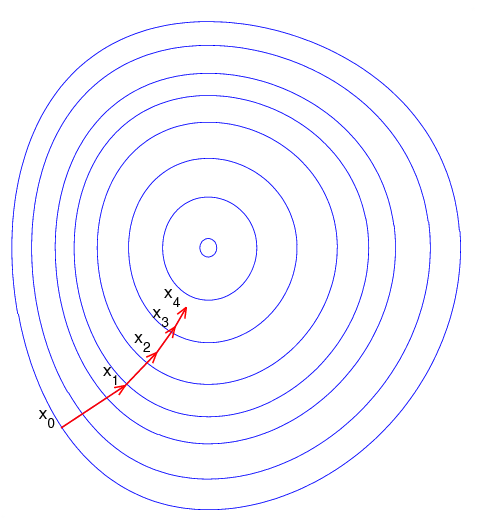
\includegraphics[width=.7\textwidth]{GradientDescent.png}

\end{frame}

\begin{frame}[fragile]
\frametitle{Newton's Method}

Newton-Raphson solves a similar problem:

\[
f(x) = 0
\]

by iterating

\[
x_{i+1} = x_i - \frac{f(x_i)}{f'(x_{i})}
\]

\note{This is equivalent to an optimization problem if we set $f'(x) = 0$.}

\end{frame}

\begin{frame}[fragile]
\frametitle{Newton's Method}

\centering
\includegraphics[width=.9\textwidth]{newton-x02.pdf}

\end{frame}

\begin{frame}[fragile]
\frametitle{Newton's Method}

\centering
\includegraphics[width=.9\textwidth]{newton-x0-4.pdf}

\end{frame}

\begin{frame}[fragile]
\frametitle{Newton's Method vs. Gradient Descent}

\centering
\includegraphics[width=.9\textwidth]{newton-vs-gd-x0-4.pdf}

\end{frame}

\begin{frame}[fragile]
\frametitle{Derivatives?}

In gradient descent, we need \alert{derivatives}. What if the function is a complex function?

\pause

\[
\frac{\partial f}{\partial x_i}(\vec{x}) = \frac{f(x_0,\cdots,x_i+h,\cdots,x_n) - f(x_0,\cdots,x_i,\cdots,x_n)}{h}.
\]

This works for very complex functions.
\end{frame}

\begin{frame}[fragile]
\frametitle{Random Greedy Hill Descent}
\begin{enumerate}
\item $x_0 \Assign ...$
\item For $i \in \{ 1, \cdots , N \}$
\begin{enumerate}
\item $C \Assign x_i + \mathcal{N}(0,\sigma)$
\item If $f(C) < f(x_i)$, then $x_{i+1} \Assign C$
\item Else $x_{i+1} \Assign x_i$
\end{enumerate}
\end{enumerate}
\end{frame}

\begin{frame}[fragile]

\centering
\includegraphics[width=.9\textwidth]{random-x02-sigma-1.pdf}

\end{frame}


\begin{frame}[fragile]

\centering
\includegraphics[width=.9\textwidth]{random-x02-sigma1.pdf}

\end{frame}

\begin{frame}[fragile]
\frametitle{In Practice}

\begin{block}{Always Use Pre-Written Functions!}
\begin{itemize}
\item They are (mostly) \alert{gradient descent} or \alert{Newton-Raphson}.
\item However, they are \alert{much better} than anything you could write\\
    (unless you spend a couple of years working on it).
\item They can fall into local minima.
\end{itemize}
\end{block}

\end{frame}

\begin{frame}[fragile]
\begin{python}
import scipy.optimize
def f(x):
    return x**4+4*x**3-4*x

print scipy.optimize.fmin(f,2.)
print scipy.optimize.fmin_cg(f,2.)
\end{python}
prints out
\begin{verbatim}
Optimization terminated successfully.
         Current function value: -1.445622
         Iterations: 17
         Function evaluations: 34
array([ 0.53212891])

Optimization terminated successfully.
         Current function value: -15.234422
         Iterations: 4
         Function evaluations: 30
         Gradient evaluations: 10
array([-2.87938508])
\end{verbatim}
\end{frame}

\begin{frame}[fragile]
\frametitle{OpenOpt}

\begin{python}
import scikits.openopt
def f(x):
    return x**4+4*x**3-4*x

P = scikits.openopt.NLP(f,2)
result = P.solve('ralg')
print 'result:', result.xf
\end{python}
\begin{verbatim}
solver: ralg   problem: unnamed   goal: minimum
 iter    objFunVal
   ...
istop:  4 (|| F[k] - F[k-1] || < ftol)
Solver:   Time Elapsed = 0.03   CPU Time Elapsed = 0.02
objFunValue: -15.234422

result: [-2.87941895]
\end{verbatim}

\end{frame}

\end{document}
